\documentclass[a4paper]{article} %可加上 twocolumn 來變成雙欄格式
\usepackage{fontspec}   %加這個就可以設定字體
\usepackage{xeCJK}       %讓中英文字體分開設置
\usepackage{indentfirst}
\usepackage{listings}
\usepackage[newfloat]{minted}
\usepackage{float}
\usepackage{graphicx}
\usepackage{caption}
\usepackage{fancyhdr}
\usepackage{hyperref}
\usepackage{amsmath}
\usepackage{multirow}
\usepackage[dvipsnames]{xcolor}
\usepackage{graphicx}
\usepackage{tabularx}
\usepackage{booktabs}
\usepackage{caption}
\usepackage{subcaption}
\usepackage{pifont}
\usepackage{amssymb}
\usepackage[backend=biber]{biblatex}
\addbibresource{main.bib}


\usepackage{pdftexcmds}
\usepackage{catchfile}
\usepackage{ifluatex}
\usepackage{ifplatform}

\usepackage[breakable, listings, skins, minted]{tcolorbox}
\usepackage{etoolbox}
\setminted{fontsize=\footnotesize}
\renewtcblisting{minted}{%
    listing engine=minted,
    minted language=python,
    listing only,
    breakable,
    enhanced,
    minted options = {
        linenos, 
        breaklines=true, 
        breakbefore=., 
        % fontsize=\footnotesize, 
        numbersep=2mm
    },
    overlay={%
        \begin{tcbclipinterior}
            \fill[gray!25] (frame.south west) rectangle ([xshift=4mm]frame.north west);
        \end{tcbclipinterior}
    }   
}

\usepackage[
top=1.5cm,
bottom=0.75cm,
left=1.5cm,
right=1.5cm,
includehead,includefoot,
heightrounded, % to avoid spurious underfull messages
]{geometry} 

\newenvironment{code}{\captionsetup{type=listing}}{}
\SetupFloatingEnvironment{listing}{name=Code}


% set the title and name
\title{VRDL HW2 Report}
\author{112550011 李佑軒}
\date{\today}


% \setCJKmainfont{Noto Serif TC}
\setCJKmainfont{Microsoft JhengHei}


\ifwindows
\setmonofont[Mapping=tex-text]{Consolas}
\fi

\XeTeXlinebreaklocale "zh"             %這兩行一定要加，中文才能自動換行
\XeTeXlinebreakskip = 0pt plus 1pt     %這兩行一定要加，中文才能自動換行

\newcommand*{\dif}{\mathop{}\!\mathrm{d}}

\begin{document}
\maketitle % write the title, name and date

\section{Introduction}

Github link: \url{https://github.com/Yu-Hsuan-1220/NYCU_Visual_Recognition_Using_Deep_Learning/tree/main/HW2}

The objective of this Lab is to develop a robust digit detection system capable of identifying and localizing numbers (0-9) in various image environments using DETR with ResNet50 backbone. The primary metric for success is the $mAP@[.5:.95]$, which requires the model to not only find the digits (Recall) but also to provide highly accurate bounding box predictions (Precision).

Our core methodology integrates the efficient local attention mechanisms of Deformable DETR with a Two-stage query initialization technique to address the inherent challenges of detecting small-scale digits within complex, noisy backgrounds. By employing multi-scale feature sampling, the model achieves heightened sensitivity to fine-grained edge details, while the two-stage mechanism provides the decoder with precise spatial priors for more stable target localization. The optimization process follows a coarse-to-fine strategy, where heavy data augmentation is initially utilized to establish robustness against environmental artifacts, followed by a refinement phase that removes these augmentations and increases the coefficients for bounding box regression losses. This strategic transition compels the model to shift from generalized regional identification to pixel-level boundary alignment, successfully bridging the performance gap between robust classification and high-precision localization. Many code implementations are inspired by the official Deformable DETR codebase \cite{Deformable_DETR_github_ref}.

\section{Method}

\subsection{Data Preprocessing}
\subsubsection{Augmentation Used}
To bridge the domain gap between our training set and the challenging inference environment, we implemented a strategic data augmentation pipeline. Given that the test data frequently contains blurry, low\-resolution, and inconsistently scaled digits, our preprocessing aims to improve the model's robustness and spatial invariance. The augmentations was carefully selected from pytorch documentation \cite{Augmentation_pytorch_ref} and tested for effectiveness.
\begin{itemize}
    \item \textbf{Scale and Crop (Resized\_Fixed):}  Our analysis indicated that the dataset is predominantly composed of small-scale objects, and the original image resolutions were often insufficient for the multi\-scale feature extraction requirements of the Deformable DETR backbone. To address this, we implemented a "scale\-then\-crop" strategy. Images were first upscaled to a dimension slightly exceeding the target resolution and subsequently cropped to the final input size (e.g., $320 \times 640$). This approach effectively "zooms in" on the objects, forcing the model to prioritize localized, fine\-grained numerical features and mitigating its reliance on global image context, which often contains misleading background artifacts.
    \item \textbf{Atmospheric \& Color Robustness:} To account for the "foggy" and blurred nature of the inference images, we applied \textbf{Gaussian Blur, Color Jitter, and Random Grayscale}. These simulate sensor noise and varying lighting conditions, ensuring the model remains discriminative even when color information is degraded or edges are indistinct.
    \item \textbf{Spatial Invariance via Translation:} We implemented \textbf{Random Translation} to artificially shift the position of digits within the frame. This prevents the model from developing a spatial bias and encourages it to search for digits across the entire image canvas.
    \item \textbf{Random Expand (Zoom-out Effect):} Since the inference dataset contains many instances where tiny digits are situated within large, complex backgrounds, we used an expansion technique. By placing the original image onto a larger, mean-filled canvas, we effectively simulated the distribution of small objects in expansive environments, improving the model's recall for distant or small-scale digits.
\end{itemize}

\subsubsection{Augmentation Not Used}
Certain standard augmentations were intentionally omitted to preserve the semantic and geometric integrity of the numerical data:
\begin{itemize}
    \item \textbf{No Horizontal Flip:} This was strictly avoided because digit detection is semantically sensitive to orientation. Flipping can fundamentally change the identity of a digit (e.g., turning a 6 into a 9 or creating non-existent characters), which would introduce significant label noise.
    \item \textbf{No Rotation:} We decided against using rotation because it often results in "vague" bounding boxes. Since the detection framework requires axis-aligned bounding boxes, rotating a tilted digit creates a significantly larger box that encompasses excessive background noise. This destroys the precision of the dataset and hinders the model's ability to achieve high $mAP_{75}$ scores.
\end{itemize}

\subsection{Model Architecture}

In this study, we transitioned from the standard DETR (DEtection TRansformer) to Deformable DETR and ultimately implemented a Two-stage Deformable DETR architecture. This progression was motivated by the specific challenges of digit detection: the high prevalence of small objects and the slow convergence rates associated with global self-attention mechanisms.

\subsubsection{Deformable DETR}
Standard DETR \cite{Standard_DETR_paper} utilizes a global self-attention mechanism, which calculates the relationship between every pair of pixels. This leads to a computational complexity of $O(N^2)$ (where $N$ is the number of pixels), making it extremely slow to train on high-resolution images. Furthermore, the global attention tends to "dilute" the signal for small objects, as the model struggles to attend to localized features amidst the vast background.

Deformable DETR \cite{deformable_DETR_paper, deformable_DETR_github} addresses these limitations by introducing the Multi-Scale Deformable Attention (MS-DeformAttn) module. Instead of attending to all pixels, each query attends only to a small, learnable set of sampling points ($k=4$ in our implementation) around a reference point across multiple feature scales.

\begin{itemize}
    \item \textbf{Efficiency:} The complexity is reduced to $O(N)$, significantly accelerating training convergence.
    \item \textbf{Small Object Performance:} By utilizing multi-scale feature maps (C3, C4, C5 in our implementation), the model can leverage higher-resolution maps (Stride 8) to capture the fine-grained details of tiny digits that are often lost in deeper, lower-resolution layers.
\end{itemize}

We utilized a ResNet-50 backbone with Frozen Batch Normalization to extract multi-scale features. To better handle small digits, we extracted three scales of feature maps with strides of 8, 16, and 32.

\begin{itemize}
    \item C3 (Stride 8): Provides the necessary spatial resolution for localized edge detection.
    \item C4 \& C5 (Strides 16/32): Provide the semantic context required for character classification.
    \item The features are projected into a hidden dimension of 256 and augmented with 2-D sine positional encodings before being fed into the transformer.
\end{itemize}

We enabled Iterative Box Refinement, where each decoder layer predicts a residual offset to the bounding box predicted by the previous layer. This allows the model to progressively "tighten" the box around the digit, which is crucial for achieving high scores in the $mAP_{75}$ metric where pixel-level precision is required.

\subsubsection{Two-stage Deformable DETR}

The most significant architectural enhancement was the implementation of the Two-stage mechanism. However, the final performance of these two architectures is roughly the same in my experiments on this task.

In the One-stage version, the decoder uses 100 static, learnable query embeddings. These queries are independent of the image content and must learn where to look through thousands of iterations. 

In our Two-stage implementation:

\begin{itemize}
    \item \textbf{Encoder Proposal Stage:} The transformer encoder processes the multi-scale features and predicts "objectness" scores and preliminary bounding boxes for every feature pixel.
    \item \textbf{Top-K Selection:} We select the top 100 highest-scoring pixels as Proposals.
    \item \textbf{Decoder Initialization:} Instead of using static embeddings, these 100 proposals are used to initialize the Reference Points and Content Queries for the decoder.
\end{itemize}
\subsection{Criterion for Training}

The core of our training logic lies in the Set-based Loss, which treats the model's predictions and the ground truth (GT) as two sets and finds the optimal "one-to-one" assignment between them.

In conventional object detectors (like YOLO), multiple anchors can be assigned to a single object, requiring NMS to filter duplicates. In our implementation, we utilize the Hungarian Algorithm (via linear\_sum\_assignment) to perform Bipartite Matching. \cite{criterion_github_ref}

This ensures that each ground truth digit is assigned to exactly one specific query. This one-to-one mapping is what allows Deformable DETR to be "NMS-free"—the model learns to suppress duplicate predictions during training because only the best-matching query receives a "positive" gradient.

To find the optimal assignment, we compute a Cost Matrix $C$ where each entry $C_{i,j}$ represents the "misalignment" between prediction $i$ and ground truth $j$:$$C = \lambda_{cls} \cdot C_{prob} + \lambda_{L1} \cdot C_{bbox} + \lambda_{giou} \cdot C_{giou}$$

\begin{itemize}
    \item \textbf{Classification Cost ($C_{prob}$):} We use the Softmax probability of the correct class. A query that identifies the digit correctly receives a lower cost.
    \item \textbf{L1 Bounding Box Cost ($C_{bbox}$):} Measures the absolute difference between the predicted and GT coordinates $(cx, cy, w, h)$.
    \item \textbf{Generalized IoU Cost ($C_{giou}$)\cite{giou_explanation}:} Since digits can be very small and may not overlap initially, standard IoU would provide zero gradients. GIoU ensures the model still receives a signal even when the boxes are far apart, encouraging them to move toward each other.
\end{itemize}

We calculate the loss only for the matched pairs (where $C_{i,j}$ is minimized) and treat unmatched predictions as negatives (background class). This encourages the model to learn precise localization and classification simultaneously, which is essential for achieving high $mAP$ scores, especially at stricter IoU thresholds.

\subsubsection{Auxiliary Loss}

Digit detection, especially for blurry and small targets, is a complex optimization problem. To stabilize and accelerate training, we utilized Auxiliary Loss (aux\_loss).

The Deformable DETR decoder consists of multiple layers (6 in our configuration). While only the final layer's output is used during inference, aux\_loss calculates the Bipartite Matching and Set Criterion for every intermediate decoder layer.

This serves as Deep Supervision, providing a training signal to early layers. It forces the model to refine its predictions layer-by-layer rather than relying solely on the final output. We found this crucial for the "Iterative Box Refinement" mechanism, as it ensures that the "offsets" being predicted are based on reasonably accurate intermediate coordinates.

\subsection{Inference}

The inference procedure was designed to maximize recall while maintaining high localization precision. Unlike traditional detectors that rely heavily on dense anchor filtering, our Deformable DETR pipeline utilizes a streamlined decoding process optimized for the sparse set of object queries.

For each test image, the model outputs 100 object queries, each consisting of a class logit vector and a bounding box coordinate. Our decoding strategy follows these steps:

\begin{itemize}
    \item \textbf{Background Exclusion:} We explicitly remove the "no-object" (background) class during the Softmax or Sigmoid calculation. By focusing only on the $K=10$ digit classes, we ensure that the model's confidence is distributed purely among the target categories.
    \item \textbf{Top-1 per Query Selection:} For each individual query, we select only the class with the highest probability (Top-1). This prevents a single query from predicting multiple overlapping labels for the same region, which simplifies the output and ensures each query acts as a unique object candidate.
\end{itemize}

We applied a relatively low score threshold of 0.01 to filter the predictions.

\begin{itemize}
    \item \textbf{The Benefit of a Low Threshold:} In the context of the $mAP$ (mean Average Precision) metric, maintaining a high recall is critical. A threshold of 0.01 allows the model to retain low-confidence detections that might otherwise be discarded. For our task, where many digits are blurry or obscured by background "cracks," this ensures that potential candidates are preserved for the final evaluation, significantly boosting the overall recall rate.
\end{itemize}


\subsection{Hyperparameter Settings and Training Details}

Our training process was divided into two distinct phases to balance the trade-off between model robustness and localization precision. We utilized the AdamW optimizer with a Cosine Annealing learning rate scheduler.

\subsubsection{Phase I: Robust Feature Exploration}

In the first phase, the model was trained for 100 epochs from scratch. The primary goal was to encourage the model to learn generalized digit features while ignoring high-frequency background noise.

\begin{itemize}
    \item \textbf{Learning Rate Strategy:} We employed a base learning rate of $1 \times 10^{-4}$ with a $10$-epoch warmup period. The backbone learning rate was set to a lower factor of $1 \times 10^{-5}$ to preserve pretrained spatial features.
    \item \textbf{Heavy Augmentation:} To prevent overfitting on the specific textures of the training images (e.g., wall cracks), we applied an aggressive augmentation suite including Random Translation, ISO Noise, and Random Expand (max ratio 0.8). This forced the model to localize digits regardless of their position or sensor noise.
    \item \textbf{Backbone Configuration:} We set freeze\_at=0 to allow the entire ResNet-50 backbone to adapt to the low-quality digit images.
\end{itemize}

\subsubsection{Phase II: High-Precision Refinement (Fine-tuning)}

After the model plateaued (around epoch 14), we initiated a refinement phase. This stage focused on "snapping" the bounding boxes to the exact boundaries of the digits to maximize the $mAP_{75}$ score.

\begin{itemize}
    \item \textbf{Clean-tuning:} We removed the heavy augmentations to provide the model with "clean" images, allowing it to focus on pixel-level boundary alignment.
    \item \textbf{Backbone Stabilization:} We increased freeze\_at to 2, freezing the shallower layers of the ResNet-50 to stabilize the feature extraction layers that had already converged.
    \item \textbf{Loss Weight Re-scaling:} We significantly increased the coefficients for localization losses. Specifically, loss\_bbox\_coef was raised from $5.0$ to $8.0$, and loss\_giou\_coef from $2.0$ to $5.0$. This prioritized the Geometric IoU and $L_1$ distance, forcing the queries to minimize even the smallest spatial offsets.
    \item \textbf{Optimization Precision:} The learning rate was reduced by 20x (to $5 \times 10^{-6}$) to perform surgical updates to the weights without disrupting the learned classification categories.
\end{itemize}

\subsubsection{Hyperparameter Settings For Two Phases}

\begin{table}[H]
\centering
\caption{Hyperparameter Settings for Phase I and Phase II}
\label{tab:hyperparameter_settings}
\begin{tabular}{lcc} % (3 columns) l: left, c: center, r: right
\toprule
\textbf{} & \textbf{Phase I} & \textbf{Phase II} \\
\midrule
Encoder Layers & 6 & 6 \\
Decoder Layers & 6 & 6 \\
Attention Heads & 8 & 8 \\
Object Queries & 100 & 100 \\
Hidden Dimension & 256 & 256 \\
Feedforward Dim & 1,024 & 1,024 \\
Feature Levels & 3 (C3, C4, C5) & 3 (C3, C4, C5) \\
Dropout & 0.1 & 0.1 \\
Optimizer & AdamW & AdamW \\
Base Learning Rate & $1 \times 10^{-4}$ & $5 \times 10^{-6}$ \\
Backbone LR & $1 \times 10^{-5}$ & $5 \times 10^{-7}$ \\
Weight Decay & $1 \times 10^{-4}$ & $1 \times 10^{-3}$ \\
Batch Size (Effective) & 16 (Total 32 via grad-acc) & 16 (Total 32 via grad-acc) \\
BBox Loss Coef ($\lambda_{L1}$) & 5.0 & 8.0 \\
GIoU Loss Coef ($\lambda_{giou}$) & 2.0 & 5.0 \\
Warmup Epochs & 10 & 0 \\
Backbone Freeze Stage & 0 (None) & 2 (Layer 0, 1, 2) \\
Augmentations & Translation, Expand, ISO Noise & Disabled (Clean-tuning) \\
\bottomrule
\end{tabular}
\end{table}

\section{Results}

\begin{figure}[H]
\centering
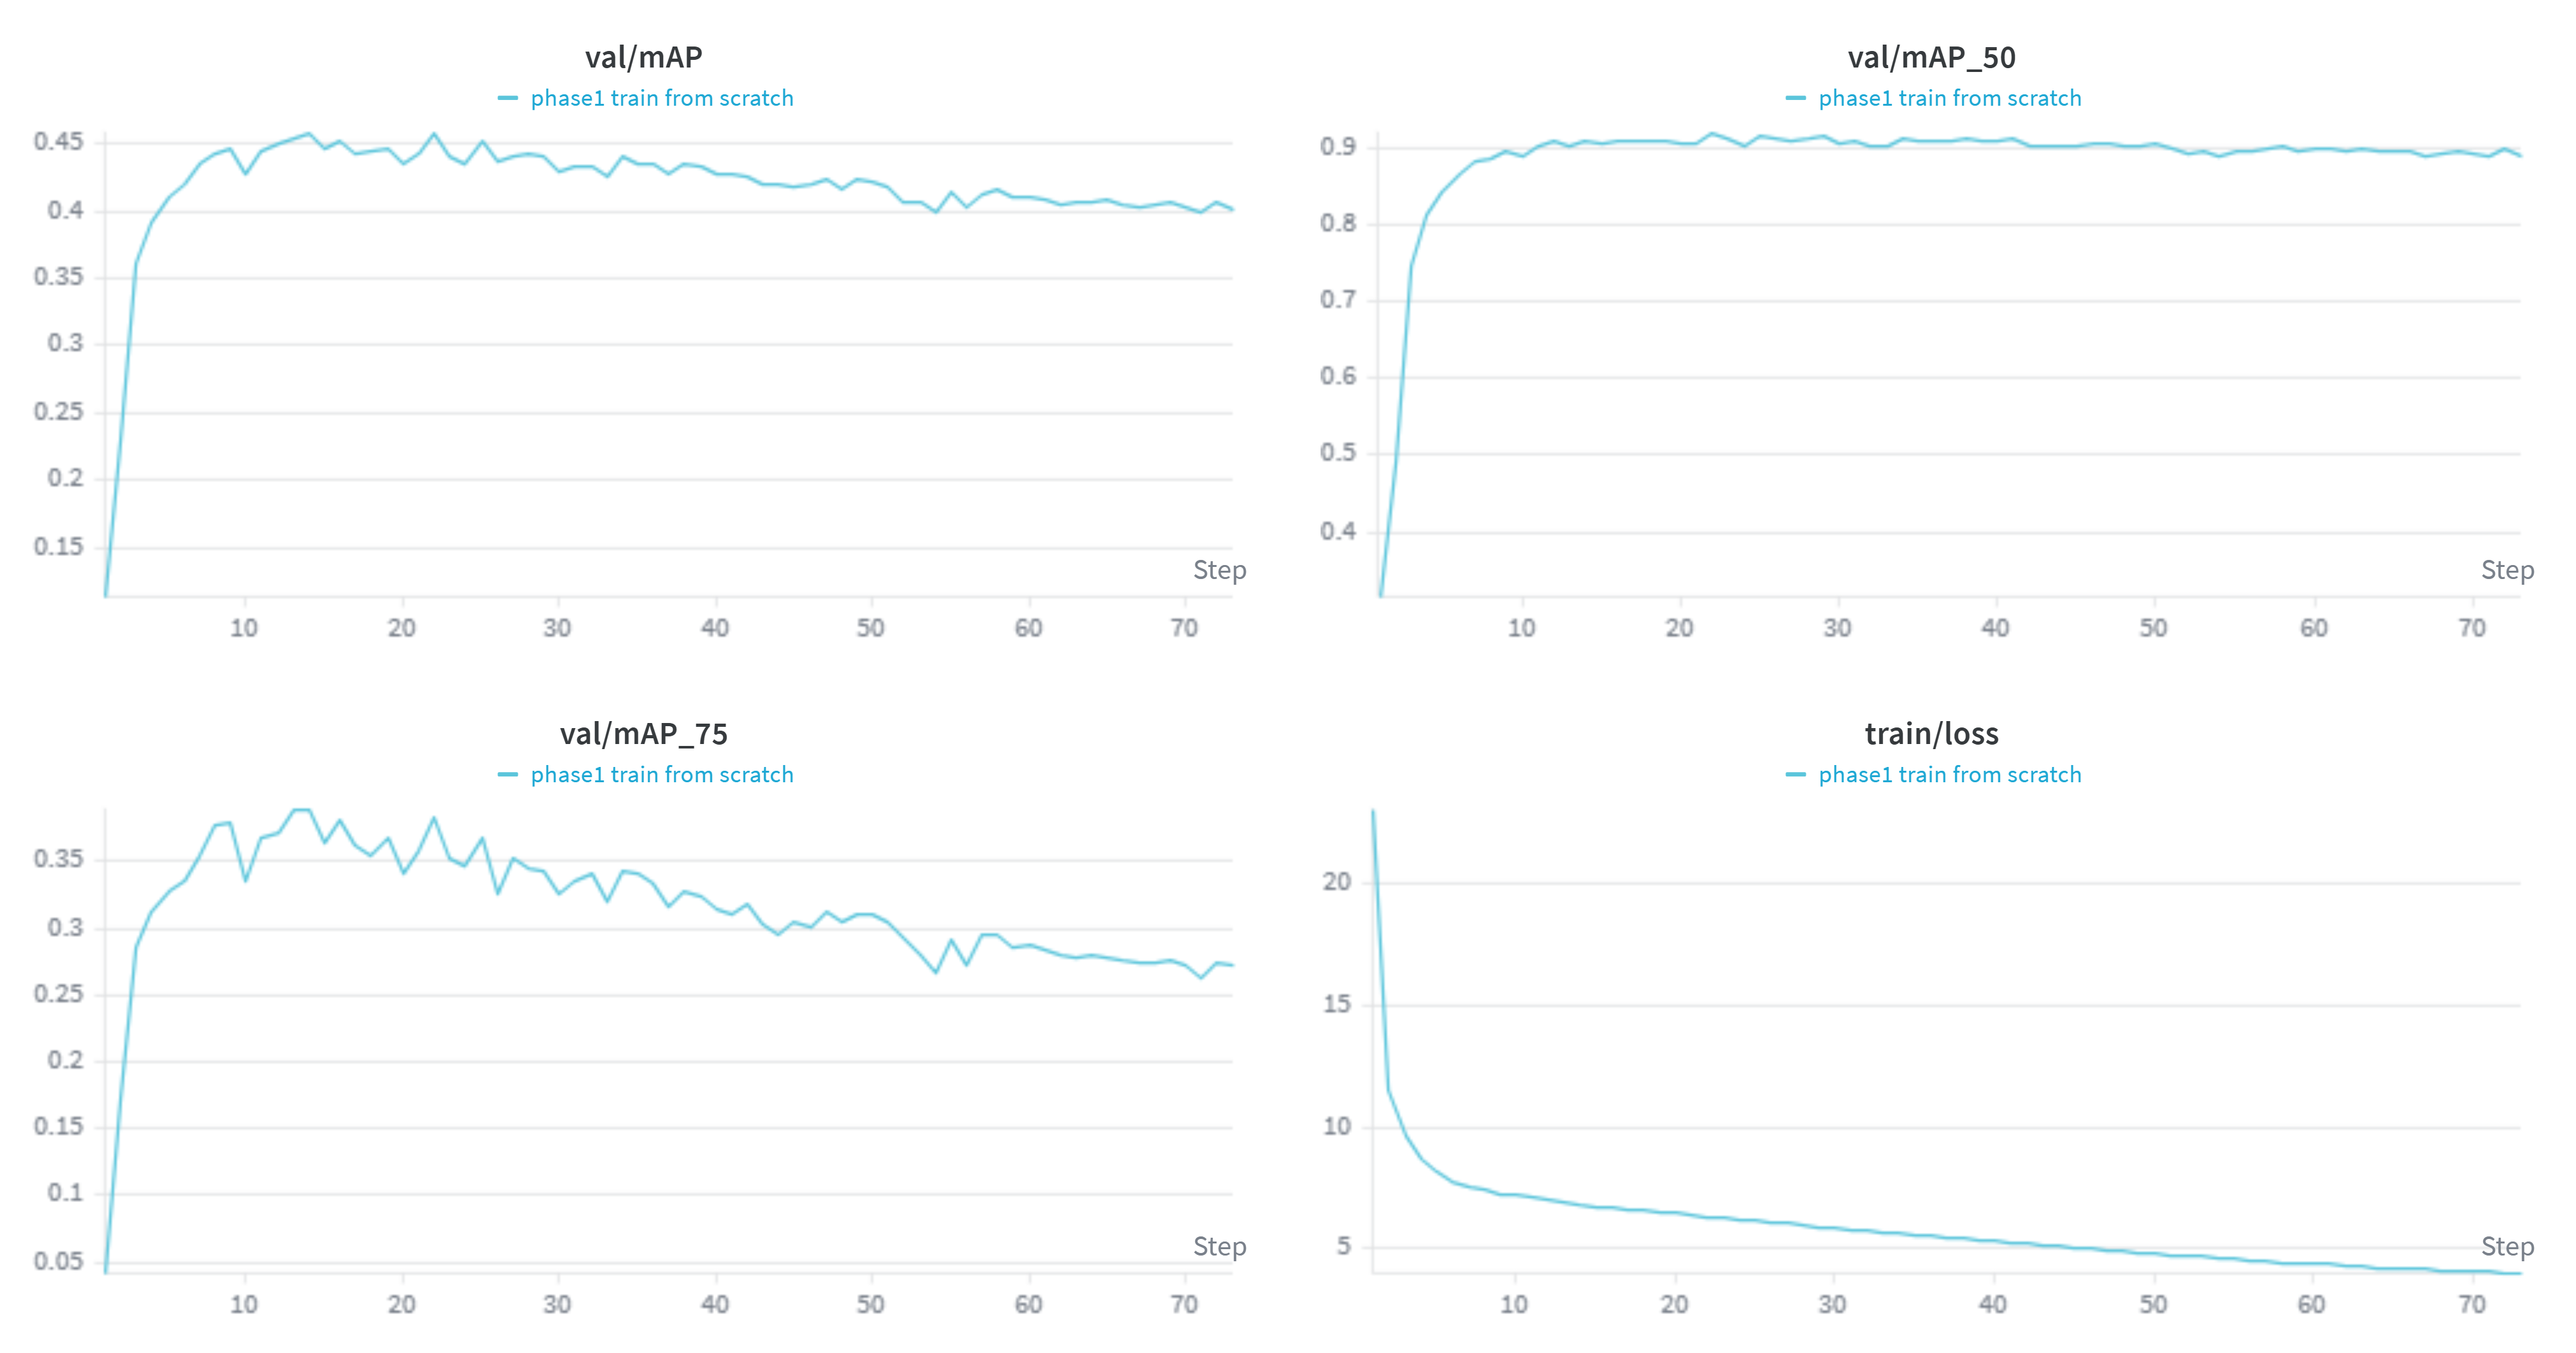
\includegraphics[width=0.95\linewidth]{figures/phase1_training_curve.png}
\caption{Phase I Training Curve}
\label{fig:phase1_training_curve}
\end{figure}

The performance of the first training phase (from scratch with heavy augmentation) provided critical insights into the model's behavior. As shown in Figure \ref{fig:phase1_training_curve}, several key trends emerged during the 100-epoch exploration phase:

A significant disparity was observed between the recognition capability and localization precision.

\begin{itemize}
    \item \textbf{$mAP_{50}$ Performance:} The model achieved an impressive $mAP_{50}$ of approximately 0.9 very early in the training process. This indicates that the Deformable DETR is highly effective at correctly identifying and categorizing digits, even under heavy data augmentation.
    \item \textbf{$mAP_{75}$ Performance:} In contrast, the $mAP_{75}$ (which requires a much higher Intersection-over-Union threshold) peaked at only 0.38. This gap suggests that while the model successfully localizes the "general area" of the digits, it struggles with pixel-level boundary alignment, likely due to the noise and blur introduced during the augmentation process.
\end{itemize}

The validation curves also exhibit a classic overfitting pattern as the training progressed:

\begin{itemize}
    \item \textbf{Training Loss vs. Validation Metrics:} While the Training Loss continued to decrease steadily (dropping from >20 to ~4), the validation scores—specifically val/mAP and val/mAP\_75—peaked around step 15 and then began a consistent decline.
    \item \textbf{Metric Degradation:} The $mAP_{75}$ score dropped from its peak of 0.38 toward 0.27 in the later stages. This confirms that the model started to over-optimize for the specific noise textures and background artifacts (such as wall cracks) present in the training set, leading to a loss of generalization on the validation set.
\end{itemize}


\begin{figure}[H]
\centering
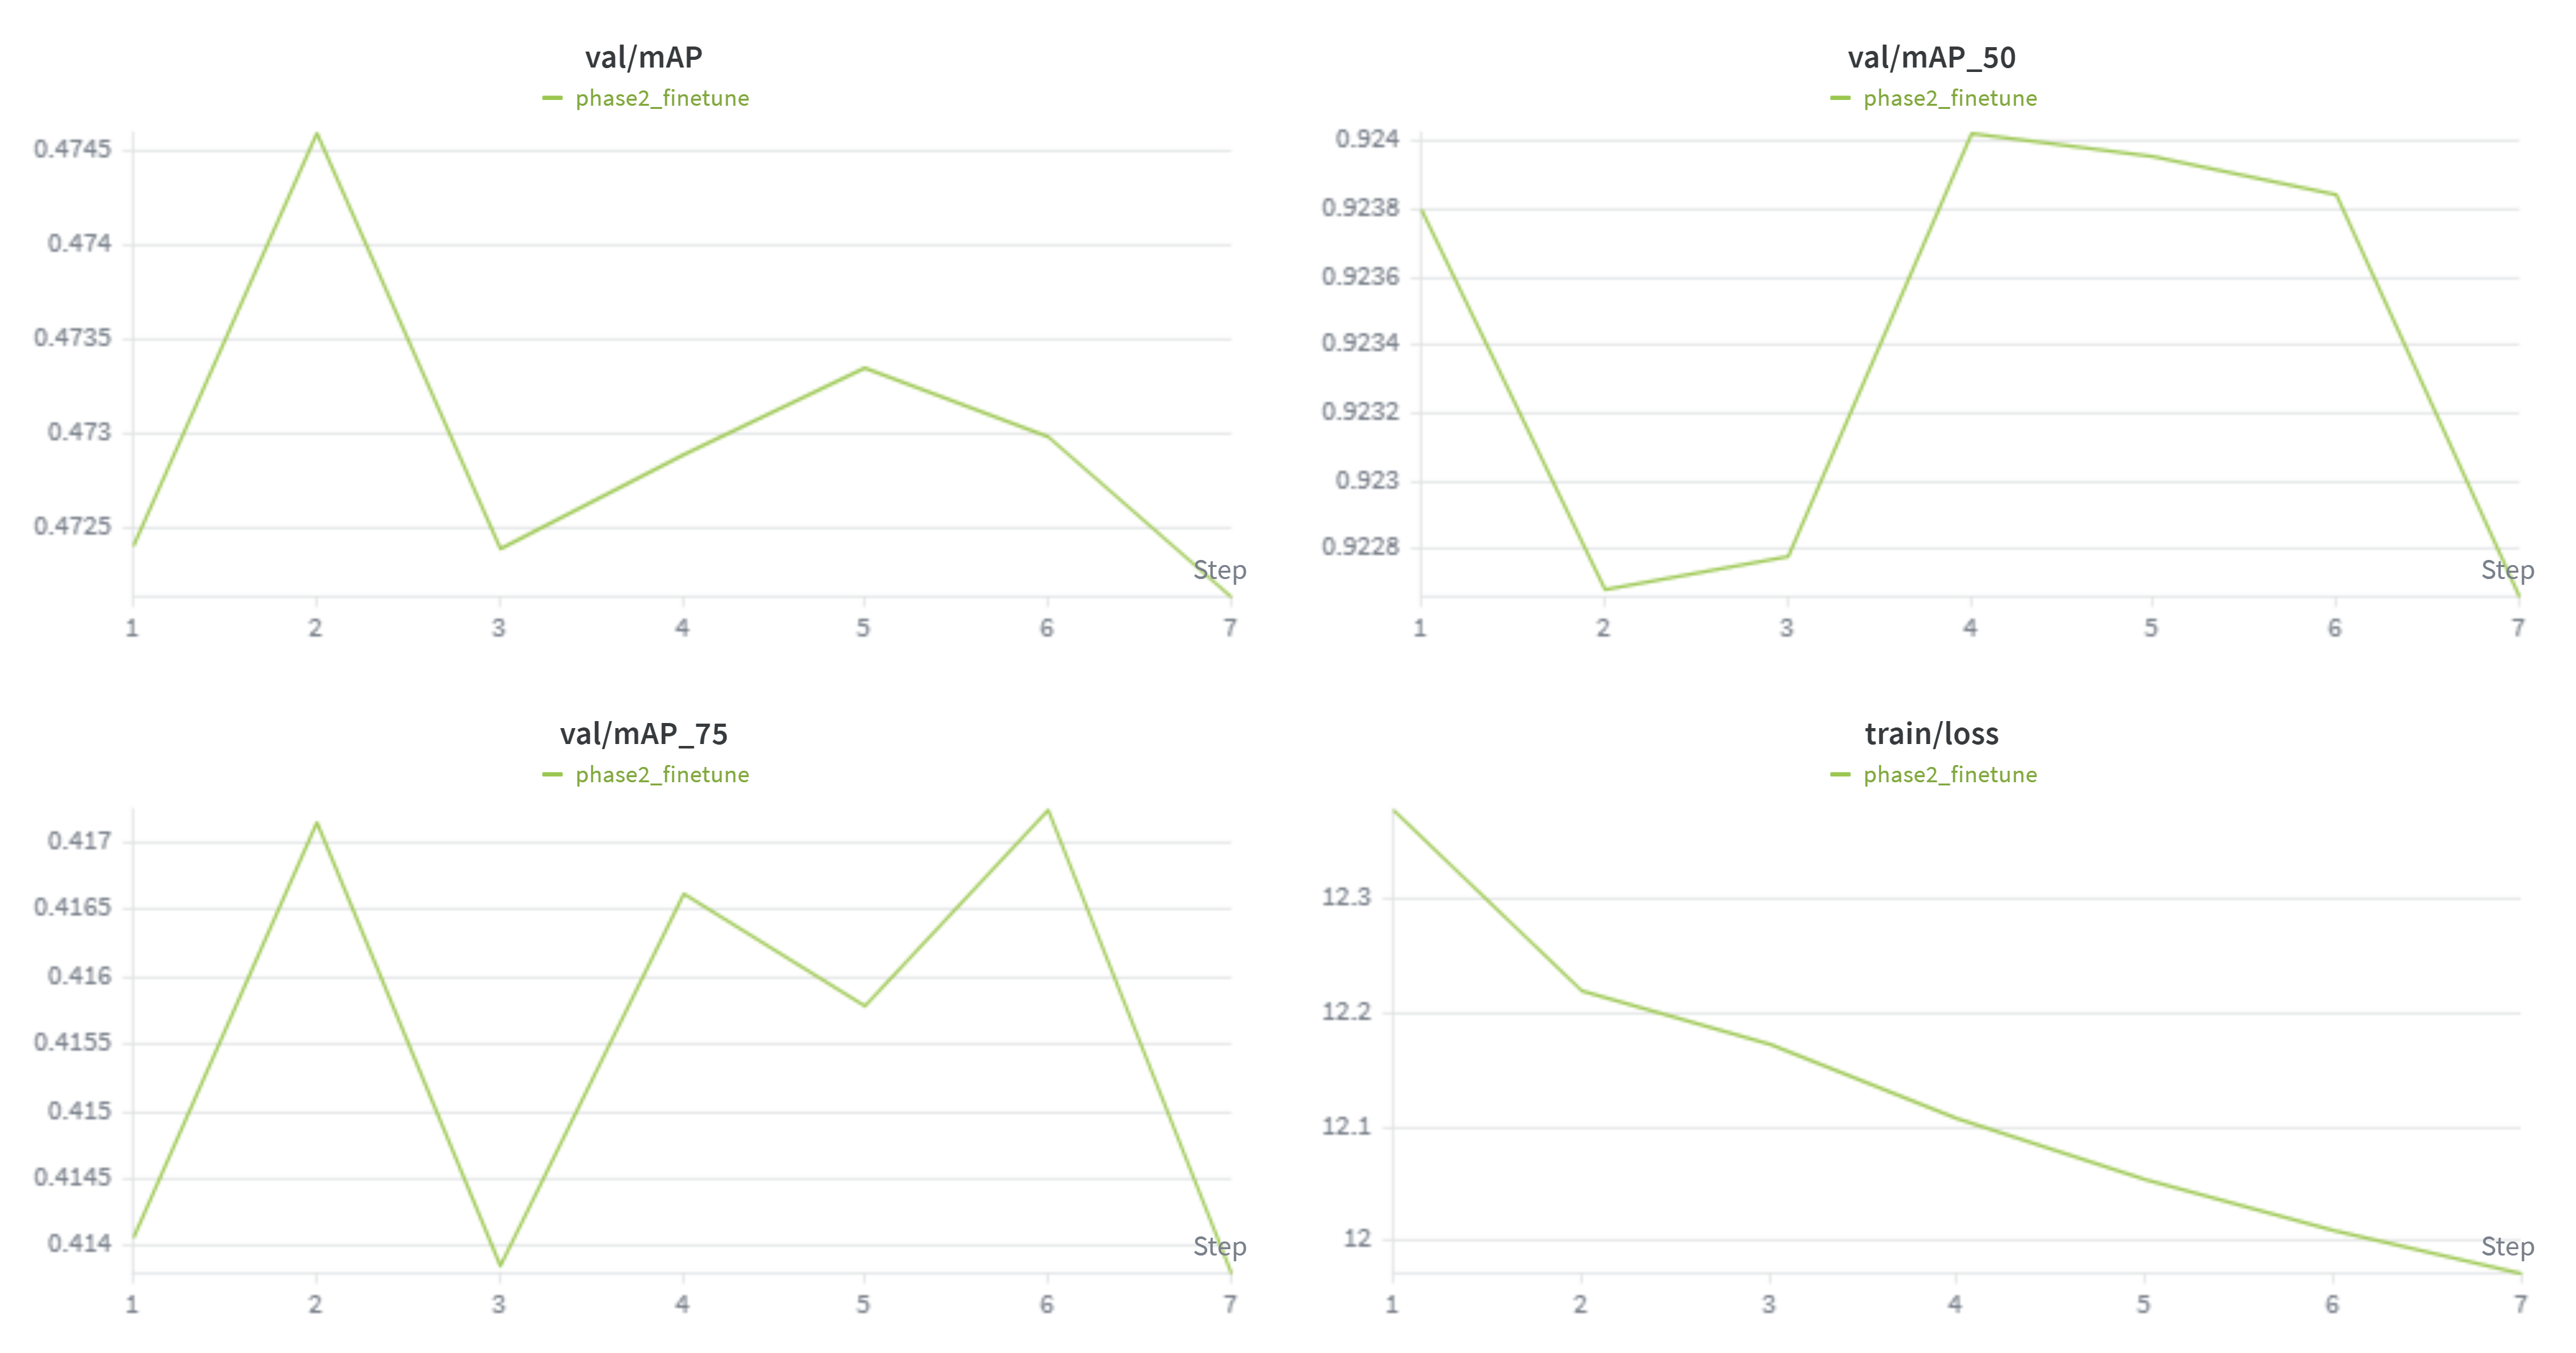
\includegraphics[width=0.95\linewidth]{figures/phase2_training_curve.png}
\caption{Phase II Training Curve}
\label{fig:phase2_training_curve}
\end{figure}

The results from Phase I indicated that continuing the initial training regime would only lead to further overfitting without improving localization precision. The primary bottleneck was identified as the trade-off between the robustness provided by heavy augmentations and the precision required for high IoU scores.

To bridge this $0.5$ mAP gap, a second phase of "Clean-tuning" was mandated. By loading the best-performing weights from Phase I (around epoch 14), removing the stochastic noise of augmentations, and re-scaling the $L_1$ and $GIoU$ loss coefficients, we aimed to "snap" the existing query predictions onto the ground truth boundaries, transforming the high $mAP_{50}$ recall into true $mAP_{75}$ precision.

As shown in Figure \ref{fig:phase2_training_curve}, after using the new training strategy and train for one epoch, mAP\_75 significantly increased from 0.38 to 0.42, which is a remarkable improvement in just one epoch. And the mAP reach the new peak of 0.4746 at epoch 2, this demonstrates that the model successfully refined its bounding box predictions to better align with the ground truth, confirming the effectiveness of the fine-tuning phase in enhancing localization precision.

\begin{figure}[H]
\centering

\includegraphics[width=0.95\linewidth]{figures/leaderboard.png}
\caption{Leaderboard Results}
\label{fig:leaderboard}
\end{figure}

After adding all the improvements such as augmentations, our final model achieved a Validation mAP of 0.47 and a Test mAP of 0.39.

\section{Additional Experiments}

To further improve the model's performance beyond the baseline Deformable DETR, we conducted a series of structural and methodological experiments. These were driven by specific hypotheses regarding the unique challenges of the blurry digit dataset.

\subsection{Structural Improvement}

\begin{figure}[H]
\centering
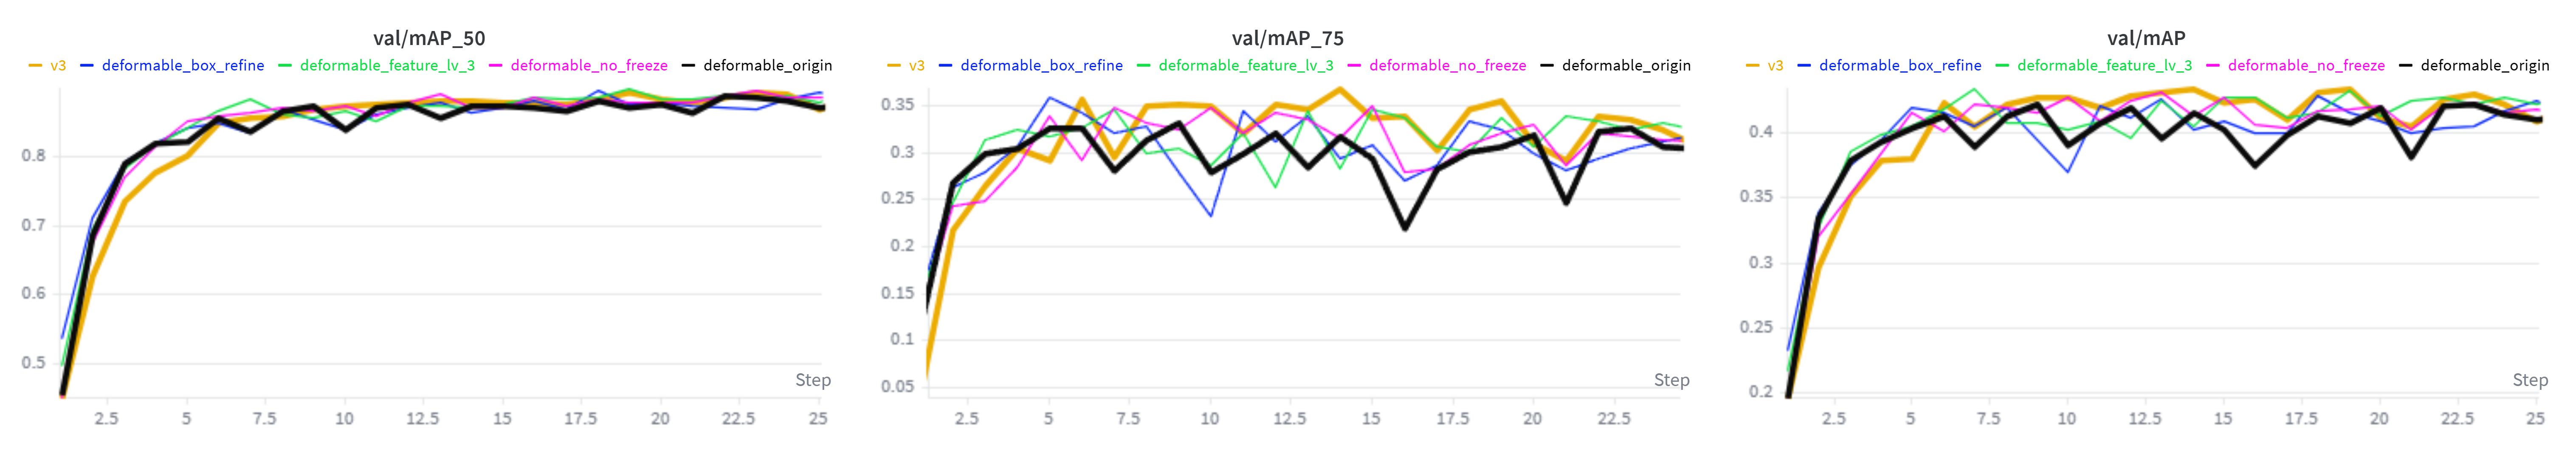
\includegraphics[width=0.95\linewidth]{figures/boxRefine_frz0_featLv3.png}
\caption{Experiment of Deformable DETR}
\label{fig:boxRefine_frz0_featLv3}
\end{figure}

From figure \ref{fig:boxRefine_frz0_featLv3}, we experiment the Deformable DETR with and without box refine, with different input feature levels to transformer, and freeze different backbone layers when training.

\textbf{Hypothesis and Methodology:}
\begin{itemize}
    \item \textbf{Full gradient flow (freeze\_at=0): } The lower layers of a ResNet-50 pretrained on ImageNet capture generic textures. However, our dataset contains specific artifacts (blurs and wall cracks) that are drastically different from ImageNet. We hypothesized that freezing the first two layers (freeze\_at=2) would limit the model's ability to extract domain-specific features. We conducted an experiment comparing freeze\_at=2 against freeze\_at=0 (unfreezing the entire backbone).
    \item \textbf{Multi-scale feature levels: } Deformable DETR typically uses four feature levels (C3, C4, C5, and a generated C6). However, for extremely small digits, a stride-64 feature map (C6) provides a resolution so low that a single pixel covers a vast area, likely introducing more background noise than useful semantic information. We restricted the multi-scale input to only C3, C4, and C5 (strides 8, 16, and 32), effectively removing the C6 level.
    \item \textbf{Iterative Box Refinement: } Standard one-step bounding box regression is insufficient for small, blurry digits where the boundary is indistinct. We hypothesized that a multi-step "coarse-to-fine" approach would allow the model to converge more accurately on high-IoU targets. We enabled the with\_box\_refine module, allowing each decoder layer to predict a residual offset based on the reference points provided by the previous layer.
\end{itemize}

\textbf{Results:} Three of the hypotheses were validated by the experiment. The mAP are more consistent and higher. The black line is the original setting of Deformable DETR, and the yellow line is the new setting with all three improvements. 

\subsection{Augmentation Improvement}

\begin{figure}[H]
\centering
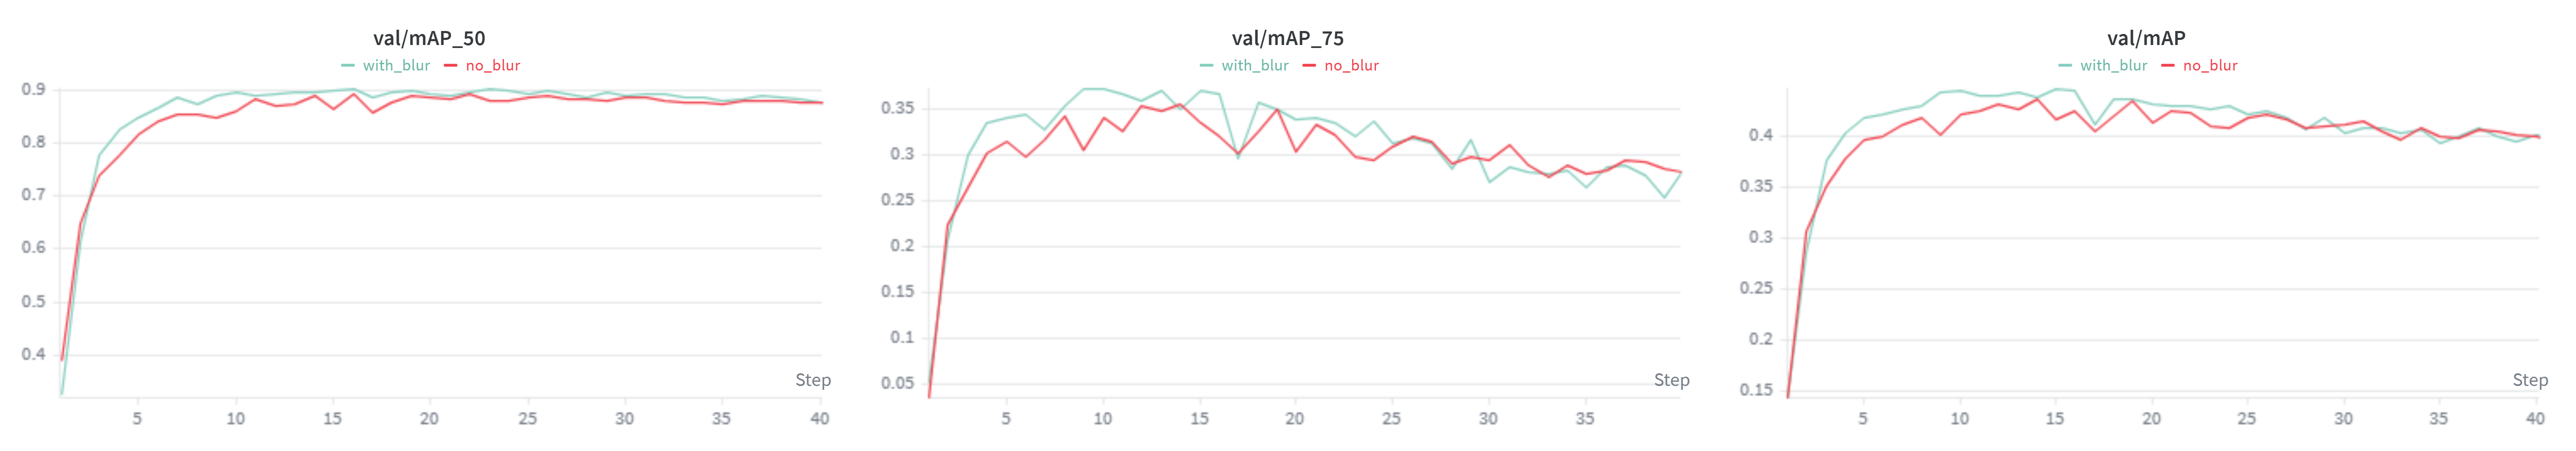
\includegraphics[width=0.95\linewidth]{figures/abla_blur.png}
\caption{Ablation Study of Gaussian Blur Augmentation}
\label{fig:abla_blur}
\end{figure}

\begin{figure}[H]
\centering
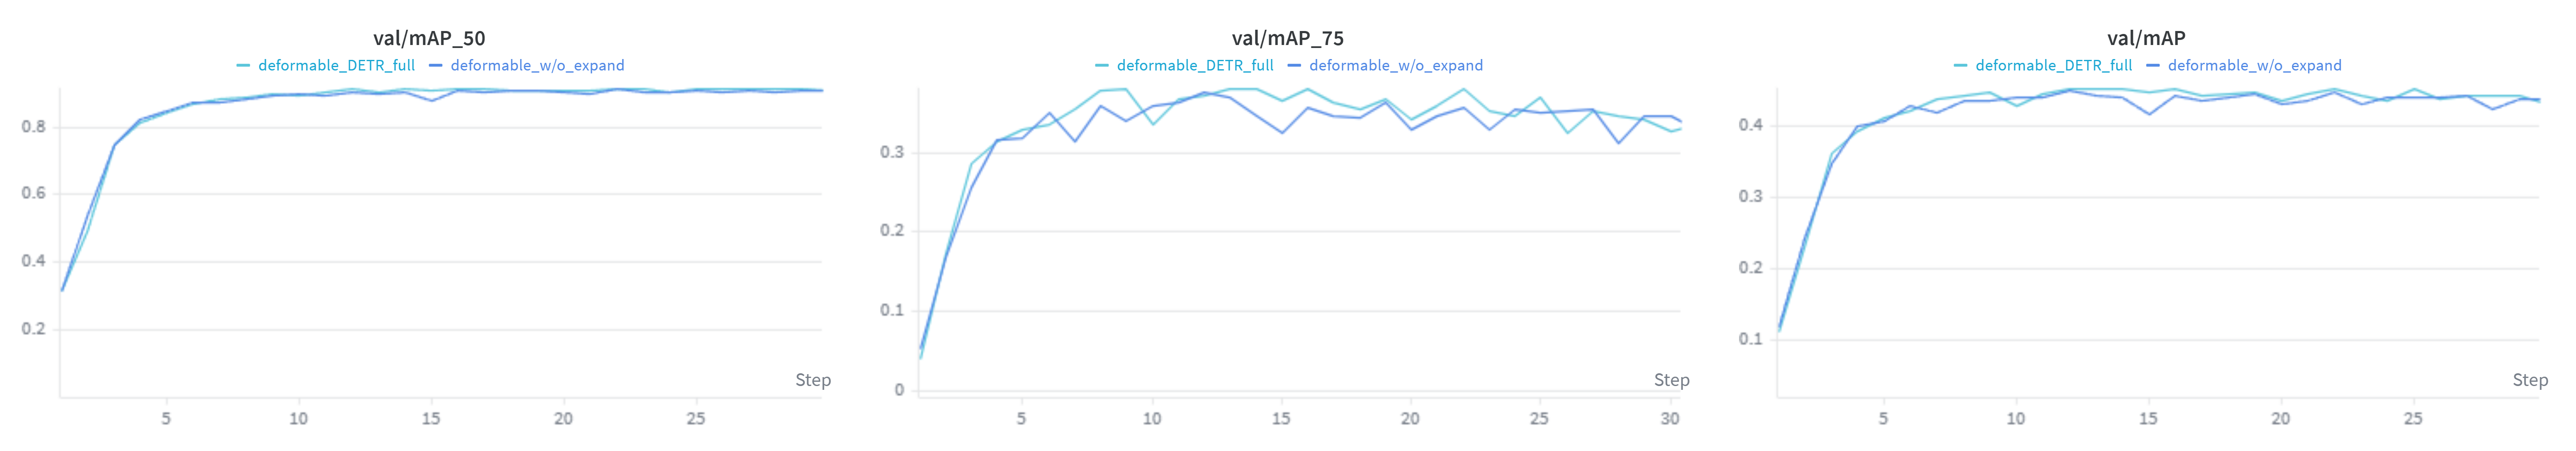
\includegraphics[width=0.95\linewidth]{figures/abla_expand.png}
\caption{Ablation Study of Expand Augmentation}
\label{fig:abla_expand}
\end{figure}

\begin{figure}[H]
\centering
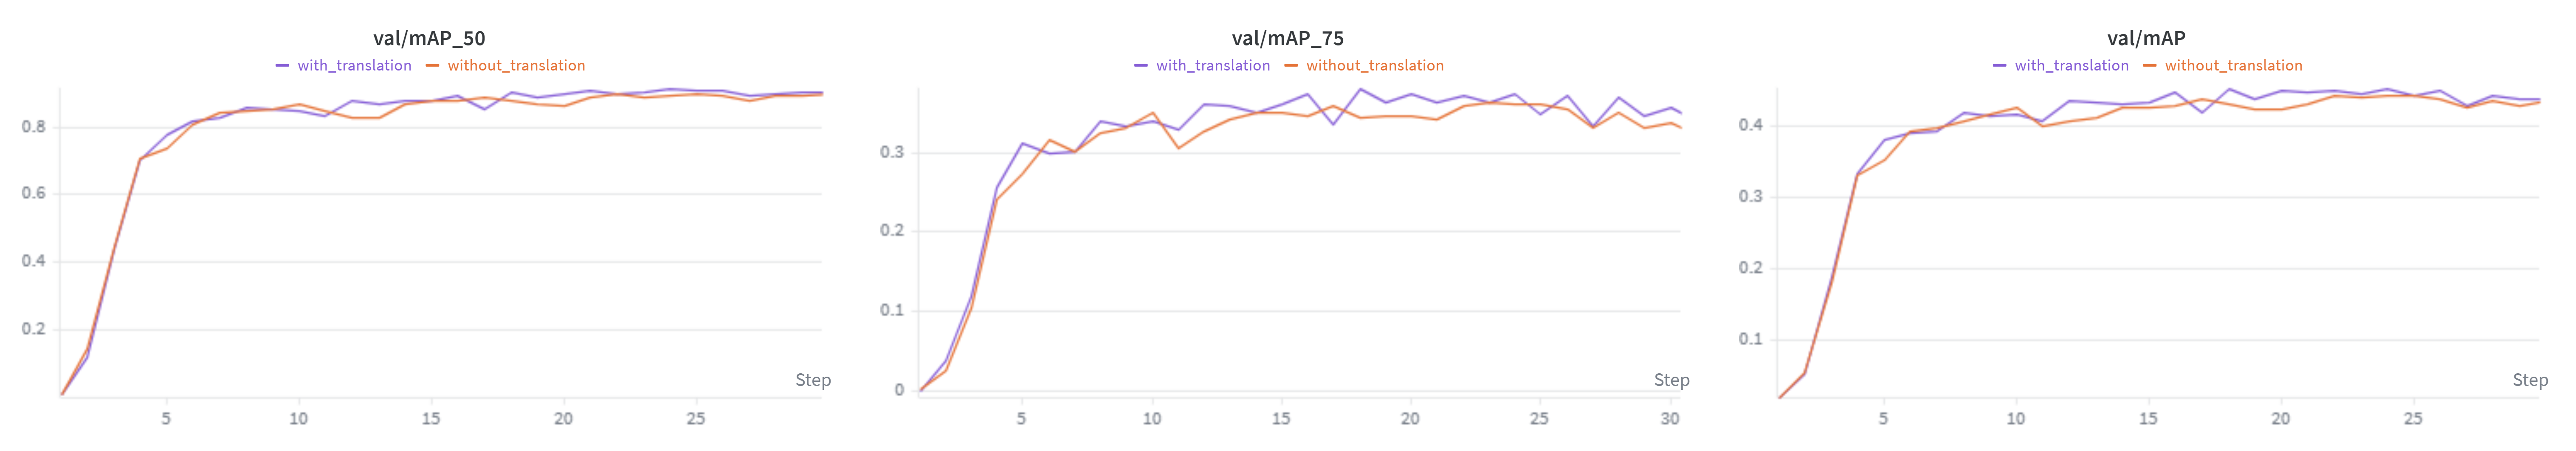
\includegraphics[width=0.95\linewidth]{figures/abla_translation.png}
\caption{Ablation Study of Translation Augmentation}
\label{fig:abla_translation}
\end{figure}

The reason why I use these augmentations are mentioned in the data preprocessing section. From figure \ref{fig:abla_blur}, \ref{fig:abla_expand} and \ref{fig:abla_translation}, we can see that all three augmentations (Gaussian Blur, Random Expand and Random Translation) contribute to the improvement of the model's performance.

A key highlight of our experimental results is the significant improvement in the model's generalization capability. While the introduction of advanced augmentations led to a higher absolute performance, its most critical impact was the reduction of the "generalization gap" between validation and test environments.

\begin{table}[H]
\centering
\caption{Gap between Validation and Test mAP with and without Augmentation}
\label{tab:gap_augmentation}
\begin{tabular}{lcc} % (3 columns) l: left, c: center, r: right
\toprule
\textbf{} & \textbf{Validation} & \textbf{Test} \\
\midrule
Without Augmentation & 0.43 & 0.33 \\
With all Augmentation & 0.47 & 0.39 \\
\bottomrule
\end{tabular}
\end{table}
This results in a performance discrepancy of only 0.08, which is a notable improvement compared to our earlier baseline models where the gap consistently exceeded 0.10. The narrowing of this gap indicates that the model is no longer merely memorizing the training/validation distribution. Instead, the heavy use of spatial and noise augmentations has forced the model to learn invariant numerical features. This enhanced robustness allows the model to better handle the domain shift and unpredictable artifacts present in the test set, ensuring reliable performance across different image qualities.

\subsection{Two-stage Deformable DETR}

\begin{figure}[H]
\centering
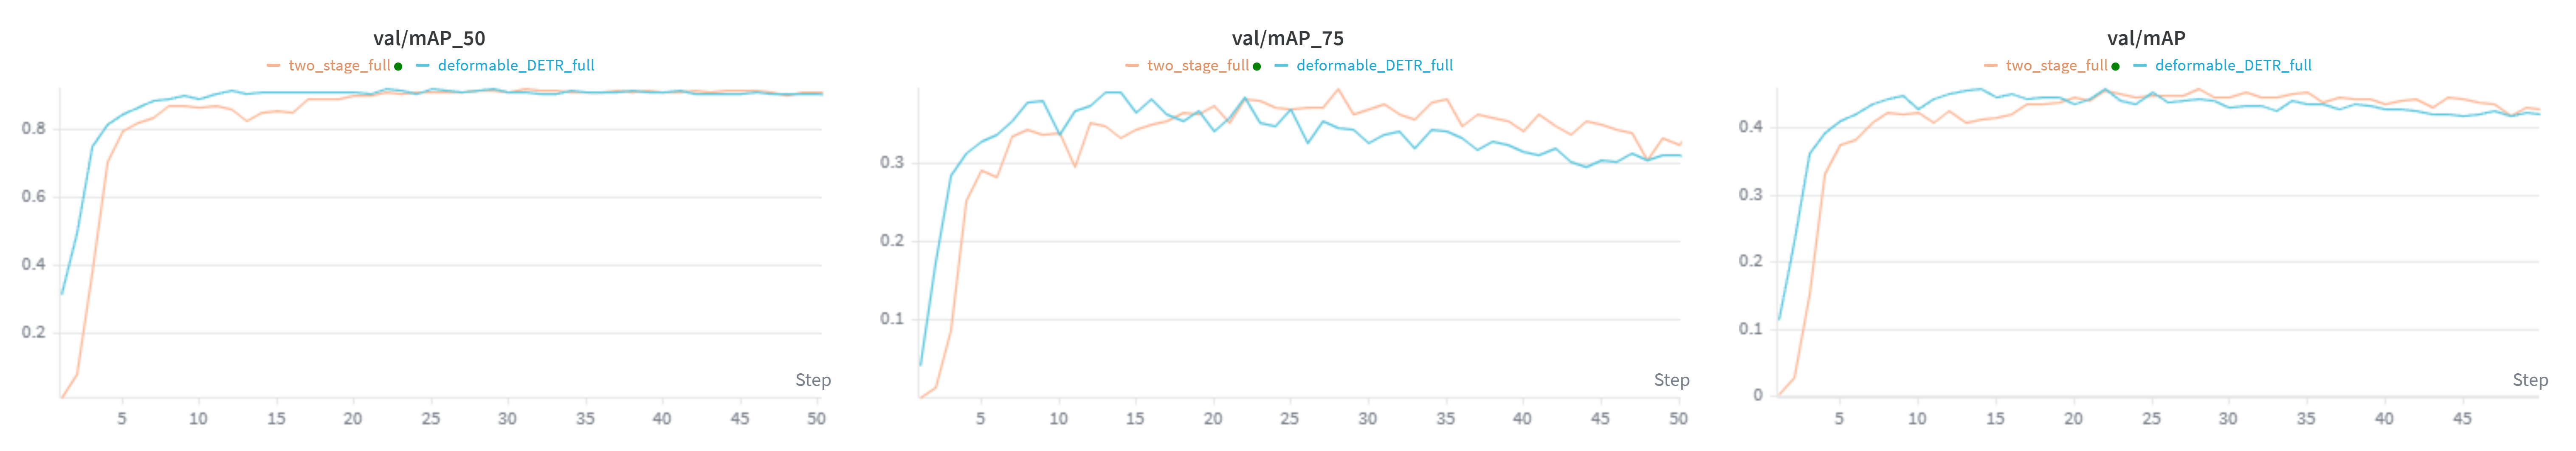
\includegraphics[width=0.95\linewidth]{figures/two_stage_deformable_DETR.png}
\caption{Comparison of Two-stage Deformable DETR}
\label{fig:two_stage_deformable_DETR}
\end{figure}

As shown in Figure \ref{fig:two_stage_deformable_DETR}, the Two-stage variant exhibits superior stability and final performance. The most notable difference is observed in the $mAP_{75}$ and total $mAP$ curves.

\begin{itemize}
    \item \textbf{Standard Deformable DETR (Blue Line): }While it converges faster in the very early steps, it exhibits significant fluctuations and a noticeable downward trend after approximately Step 20. This suggests that the model's static queries are susceptible to "distraction" by background artifacts, leading to unstable localization.
    \item \textbf{Two-stage Deformable DETR (Orange Line): }The training trajectory is considerably smoother and maintains a higher performance plateau. This stability is attributed to the Encoder-proposal mechanism, which filters out the majority of background noise before the decoder even begins its task. By starting with high-quality, image-dependent proposals, the optimization landscape for the decoder becomes much more well-behaved.
    \item While both models reach a similar ceiling in $mAP_{50}$ (~0.9), the Two-stage model consistently outperforms the one-stage baseline in $mAP_{75}$.
\end{itemize}

However, I cannot find out a way to further finetune the Two-stage model to achieve higher mAP. So the final submission is still based on the One-stage Deformable DETR, which has a slightly higher mAP after finetuning than the Two-stage version in my experiments.

% \begin{figure}[H]
% \centering
% \includegraphics[width=0.95\linewidth]{figures/chaewon.jpg}
% \caption{Example of figure of my wife}
% \label{fig:my_wife}
% \end{figure}

% we can reference the figure \autoref{fig:my_wife}

\printbibliography % to print the bibliography
\end{document}